\textbf{COLUNI 2022 -- Questão 04}\par\medskip Leia o texto a seguir para as questões 03 e 04.

\par

% COLUNI-AUTO-FIGURES-BEGIN
\begin{figure}[htbp]
\centering
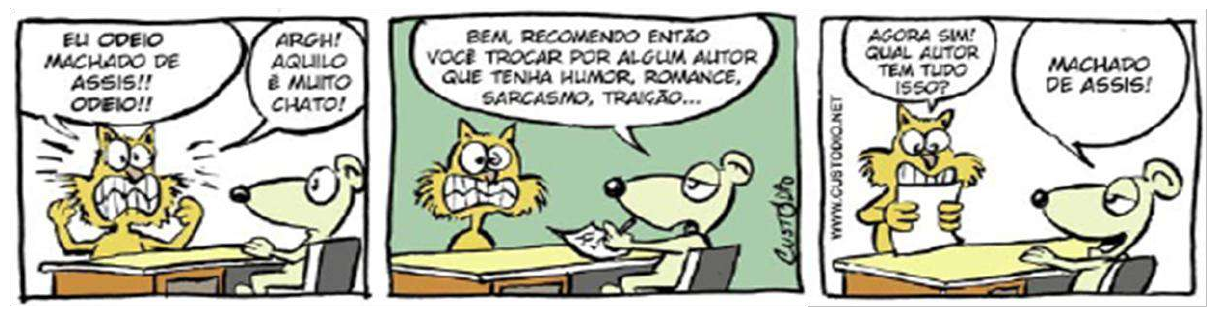
\includegraphics[width=0.95\linewidth]{static/simulados/coluni/figuras/2022/questao-04/figura-1.png}
\end{figure}
% COLUNI-AUTO-FIGURES-END

Disponível em: https://enem.estuda.com/questoes/?id=399426 tirinhas+de+literatura\&tbm=isch\&source. Acesso em: 31 ago. 2021.

\par

As formas verbais \underline{odeio}, \underline{é}, \underline{tenha} e \underline{tem} estão flexionadas, respectivamente, nos modos:


\begin{enumerate}
\item subjuntivo, subjuntivo, imperativo, indicativo.
\item indicativo, indicativo, subjuntivo, indicativo.
\item indicativo, subjuntivo, indicativo, indicativo.
\item subjuntivo, imperativo, indicativo, subjuntivo.\end{enumerate}
